\documentclass{article}
\usepackage{amsmath}
\usepackage{amssymb}
\usepackage{graphicx}
\usepackage{hyperref}
\usepackage[version=4]{mhchem}


\begin{document}
As shown in the figure, \(\angle A B D=\angle A C D=60^{\circ} . \angle A D B=90^{\circ}-\frac{1}{2}\) \(\angle B D C\). Show that triangle \(A B C\) is an isosceles triangle.

Solution:
Method 1:\\
Since \(\angle A B D=\angle A C D=60^{\circ}\), points \(A, B, C\), and \(D\) are concyclic. Therefore,\\
\centering
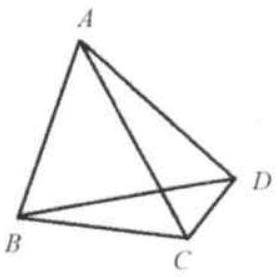
\includegraphics[width=\textwidth]{images/196(2).jpg}\\
\(\angle A D B=\angle A C B=\alpha ; \angle D B A=\angle D A C=\beta ; \angle B A C=\angle B D C=\gamma\).\\
\(\beta+\gamma+60^{\circ}+\alpha=180^{\circ}\)\\
We know that \(\angle A D B=90^{\circ}-\frac{1}{2} \angle B D C\) or\\
\(\alpha=90^{\circ}-\frac{1}{2} \gamma \Rightarrow \quad 2 \alpha+\gamma=180^{\circ}\)\\
(1) \(+\alpha: \beta+\gamma+60^{\circ}+2 \alpha=180^{\circ}+\alpha\)\\
\centering
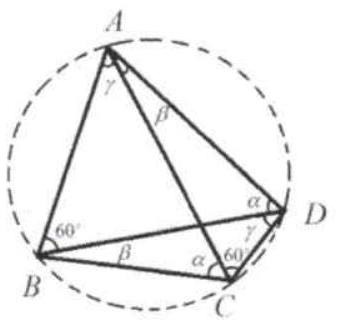
\includegraphics[width=\textwidth]{images/196(3).jpg}


Substituting (2) into (3): \(\beta+60^{\circ}+180^{\circ}=180^{\circ}+\alpha \quad \Rightarrow \quad \beta+60^{\circ}=\alpha\). That is \(\angle A B C=\angle A C B\), triangle \(A B C\) is an isosceles triangle.

Method 2:\\
Extend \(A D\) and \(B C\) to meet at \(E\).\\
Since \(\angle A B D=\angle A C D=60^{\circ}\), points \(A, B, C\), and \(D\) are concyclic.\\
Therefore,\\
\(\angle C D E=\angle A B C, \angle A C B=\angle A D B\).\\
\centering
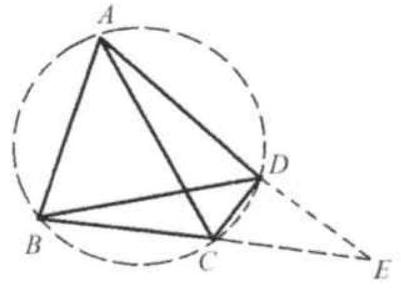
\includegraphics[width=\textwidth]{images/197.jpg}

We know that \(\angle A D B=90^{\circ}-\frac{1}{2} \angle B D C\) or\\
\(2 \angle A D B=180^{\circ}-\angle B D C \quad\) or \(\quad \angle A D B+\angle A D B+\angle B D C=180^{\circ}\)\\
But\\
\(\angle C D E+\angle A D B+\angle B D C=180^{\circ}\)\\
So \(\angle A D B=\angle E D C\)\\
That is \(\angle A B C=\angle A C B\), triangle \(A B C\) is an isosceles triangle\\

\end{document}
